\section{Results}

\subsection*{Training the Convolutional Neural Network}
\qquad The dataset, CBIS-DDSM (Curated Breast Imaging Subset of the Digital Database for Screening Mammography), was downloaded from TCIA (The Cancer Imaging Archive). The dataset downloaded was similar to that in Shen's study \cite{CNNmodel}. But, instead of the whole-image dataset version of CBIS-DDSM, the dataset downloaded was the cropped region of interest (ROI) version.

\subsubsection{Preparing the Dataset}
\qquad Preparing the dataset was no easy task, for the dataset was erroneous. For context, there are two file locations in the given CSV metadata file for the whole dataset: one for the cropped ROI, and the other for the ROI mask. There are several occurences where the file location of the cropped ROI was mislabeled and would point to the ROI mask instead. Since there are several occurences in the dataset's metadata where file locations are erroneous, there is no way of confirming if the other information are erroneous as well. This poses a potential problem where the ROIs are misclassified. It is this for this reason that the erroneous instances are kept track of.
	
\subsubsection{Setting the Hyperparameters}	
\qquad After setting the proper number of epochs, learning rate, batch size, and the optimizer namely Nesterov Gradient Descent seen in figure \ref{fig:hyperparameters} as well as utilizing a pre-trained ResNet-50 model, and having the model undergo initial training, the model looked promising as it slowly converges shown in figure \ref{fig:firstModelLog1} for the first few iterations and figure \ref{fig:firstModelLog2} for the last remaining iterations. However, after having the model tested, it only attained an accuracy of 33\% as it correctly labeled 243 images from a test set of 704. A possible cause for such a low accuracy is the lack of data augmentation techniques applied on the dataset used. Another cause is the imbalanced number of instances per category specifically there are 681 ROI images for benign mass, 637 ROI images for malignant mass, 1,002 ROI images for benign calcification, and 544 ROI images for malignant calcification.

\begin{figure}[h]
	\centering
  	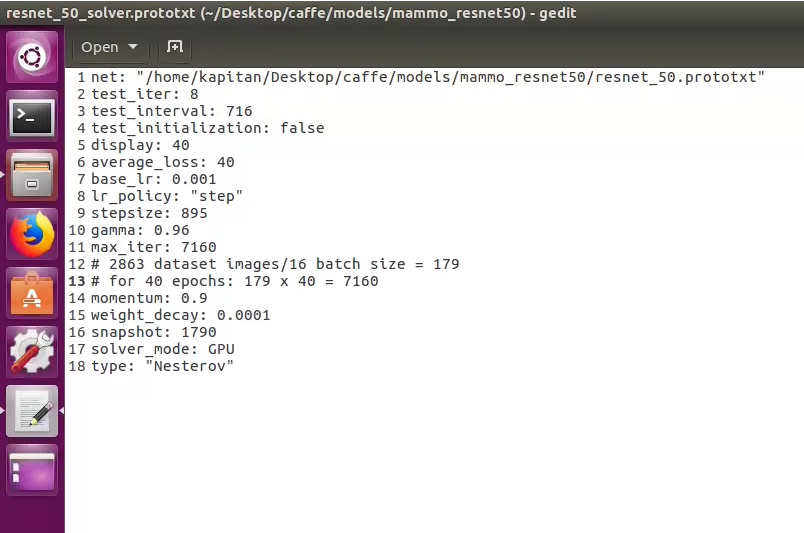
\includegraphics[scale=0.6]{images/hyperparameters.png}
	\caption{ResNet-50's hyperparameters, Mammo}
  	\label{fig:hyperparameters}
\end{figure}

\begin{figure}[h]
	\centering
  	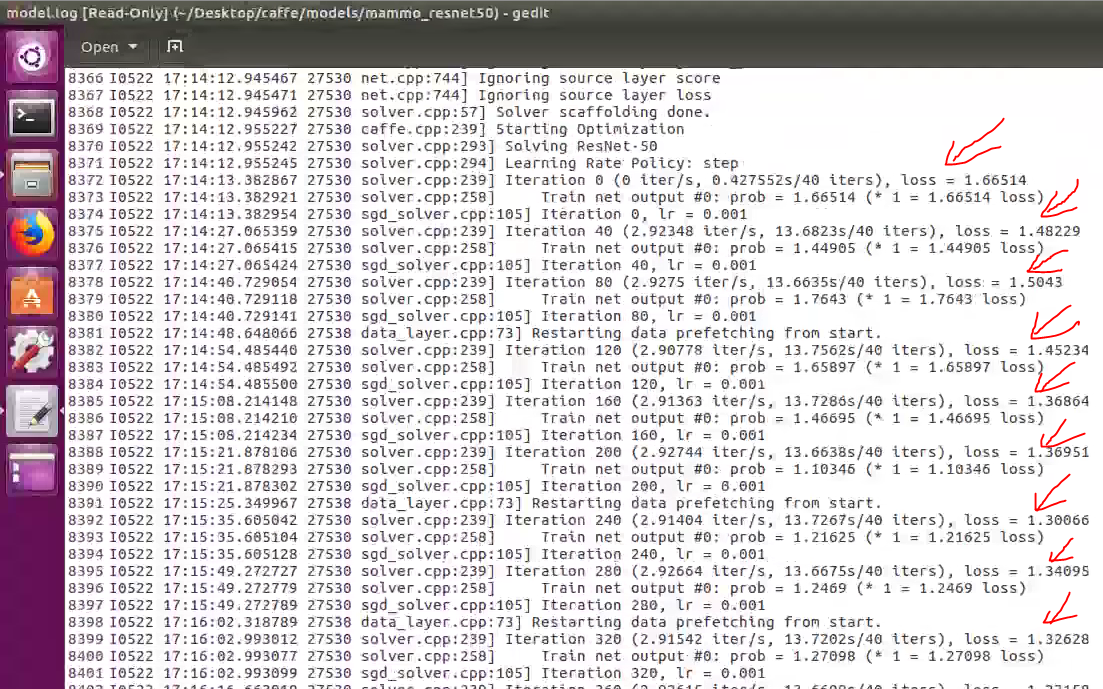
\includegraphics[scale=0.5]{images/firstModelLog.png}
	\caption{The log file of the model showing diminishing loss on the first few iterations as indicated by the red arrows, Mammo}
  	\label{fig:firstModelLog1}
\end{figure}

\begin{figure}[h]
	\centering
  	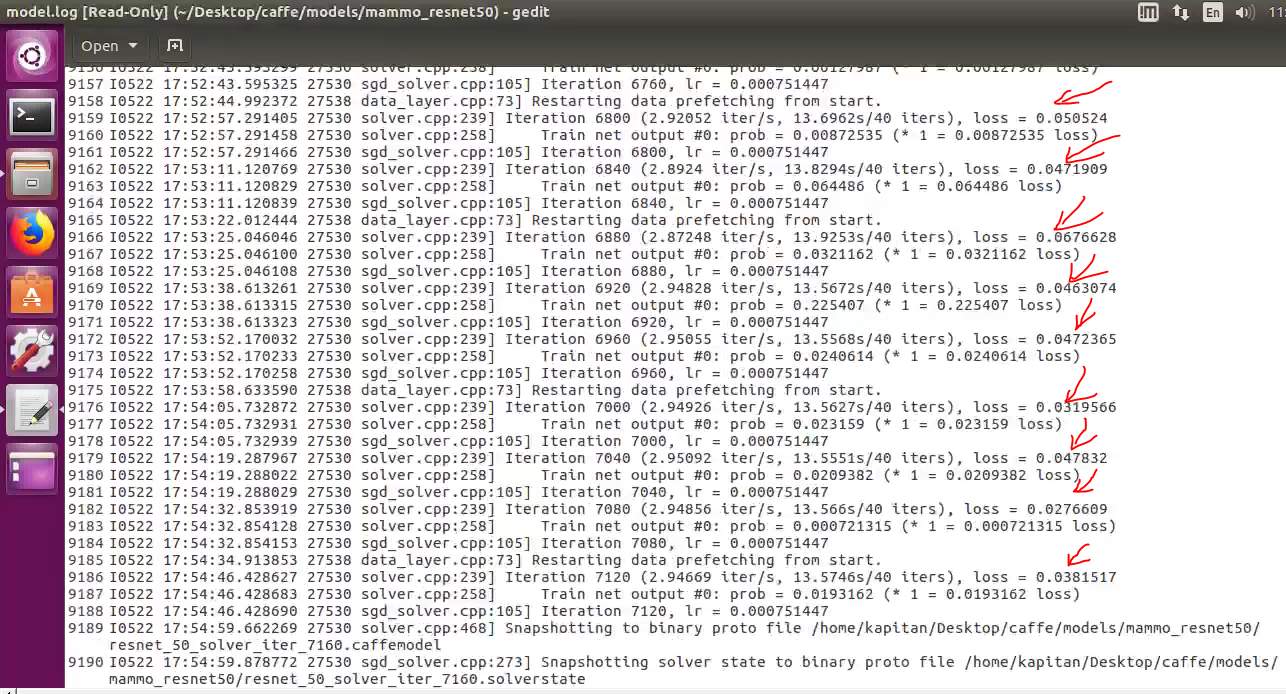
\includegraphics[scale=0.5]{images/firstModelLog2.png}
	\caption{The log file of the model showing diminishing loss on the last remaining iterations as indicated by the red arrows, Mammo}
  	\label{fig:firstModelLog2}
\end{figure}

\subsubsection{Improving the Accuracy}
\qquad To address the low accuracy, the dataset was balanced having the number of images under each category set at a maximum of 544 ROI images. This was done by removing the extra erroneous instances from each category, and then randomly removing other ones until it reached 544 images except images under malignant calcification. Then the model was trained again with the same hyperparameters except for the number of epochs which was increased from 40 to 50, and the use of the balanced dataset. Figures \ref{fig:secondModelLog1} and \ref{fig:secondModelLog2} show the model's convergence at the first few iterations, and at the last remaining iterations. The accuracy improved up to 43\% with the model correctly classifying 305 images out of 704 as seen in figure \ref{fig:secondModelAccuracy}.

\begin{figure}[h]
	\centering
  	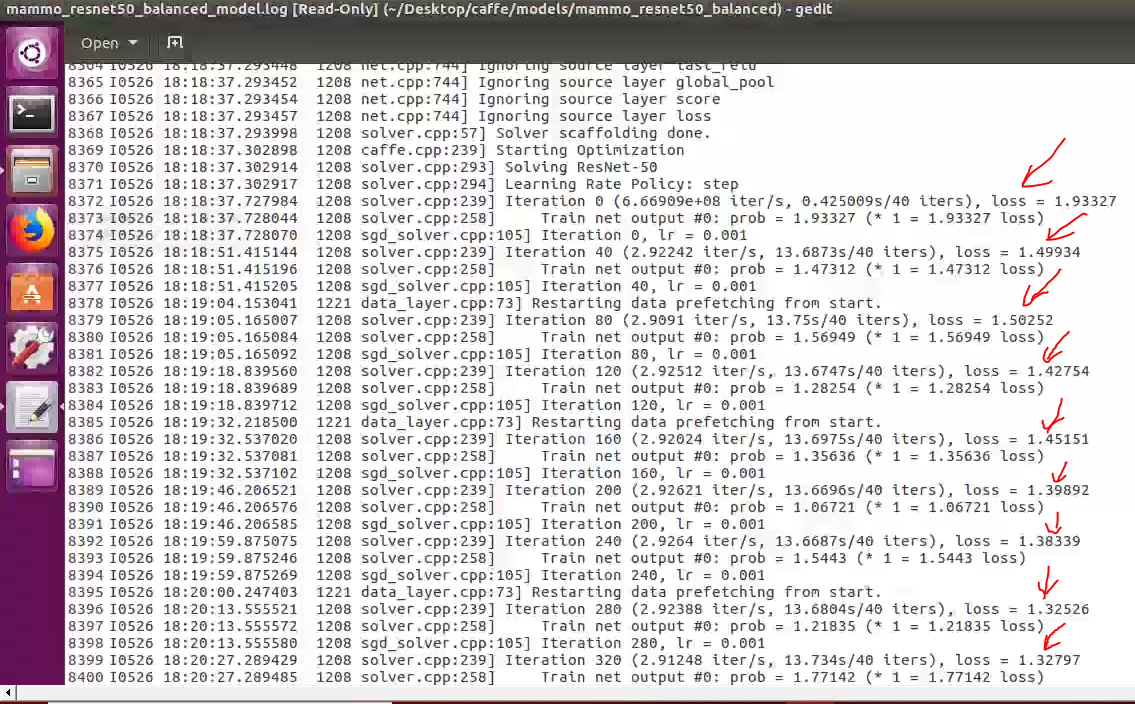
\includegraphics[scale=0.5]{images/secondModelLog.png}
	\caption{The log file of the model with the balanced dataset diminishing improving loss on the first few iterations as indicated by the red arrows, Mammo}
  	\label{fig:secondModelLog1}
\end{figure}

\begin{figure}[h]
	\centering
  	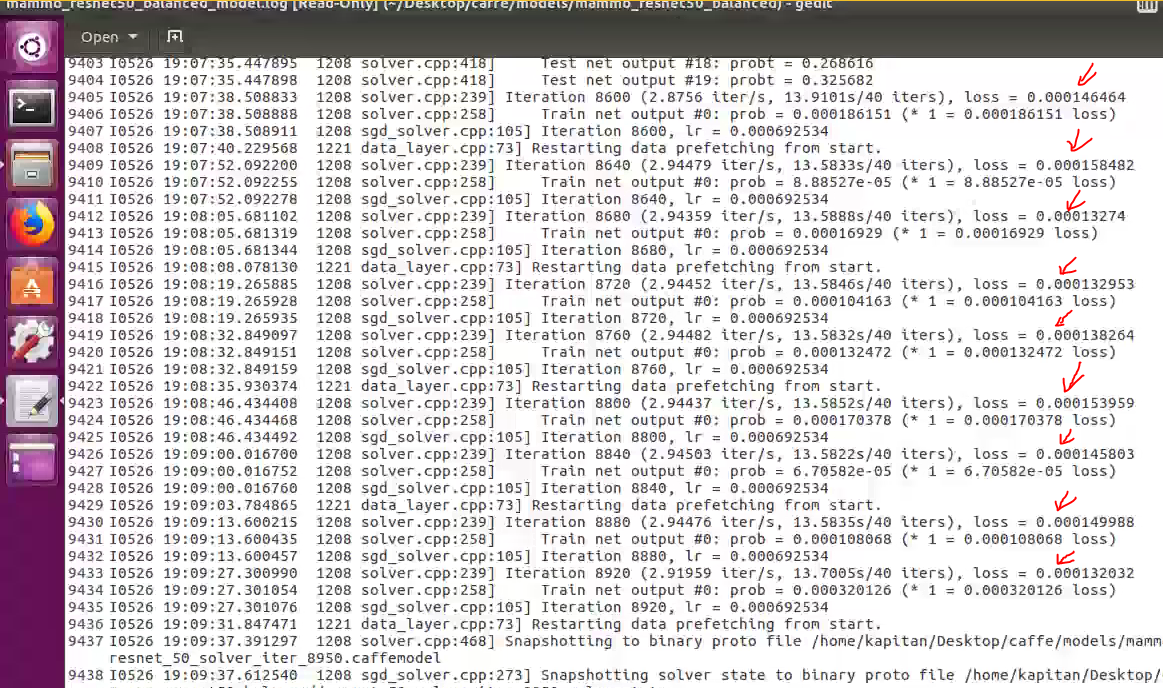
\includegraphics[scale=0.5]{images/secondModelLog2.png}
	\caption{The log file of the model with the balanced dataset diminishing improving loss on the last remaining iterations as indicated by the red arrows, Mammo}
  	\label{fig:secondModelLog2}
\end{figure}

\begin{figure}[h]
	\centering
  	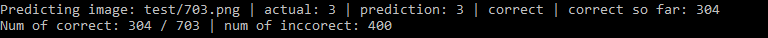
\includegraphics[scale=0.5]{images/secondModelAccuracy.png}
	\caption{The accuracy of the model after balancing the dataset, Mammo}
  	\label{fig:secondModelAccuracy}
\end{figure}
	
\subsection*{General User Functionalities}
\qquad The home page of the system is seen in  figure \ref{fig:mammoHome}. A basic description of what the site is for is present here along with the features it has to offer. Also, a navbar that provides the user access to the site's features is present at all pages of the site.

\begin{figure}[h]
	\centering
  	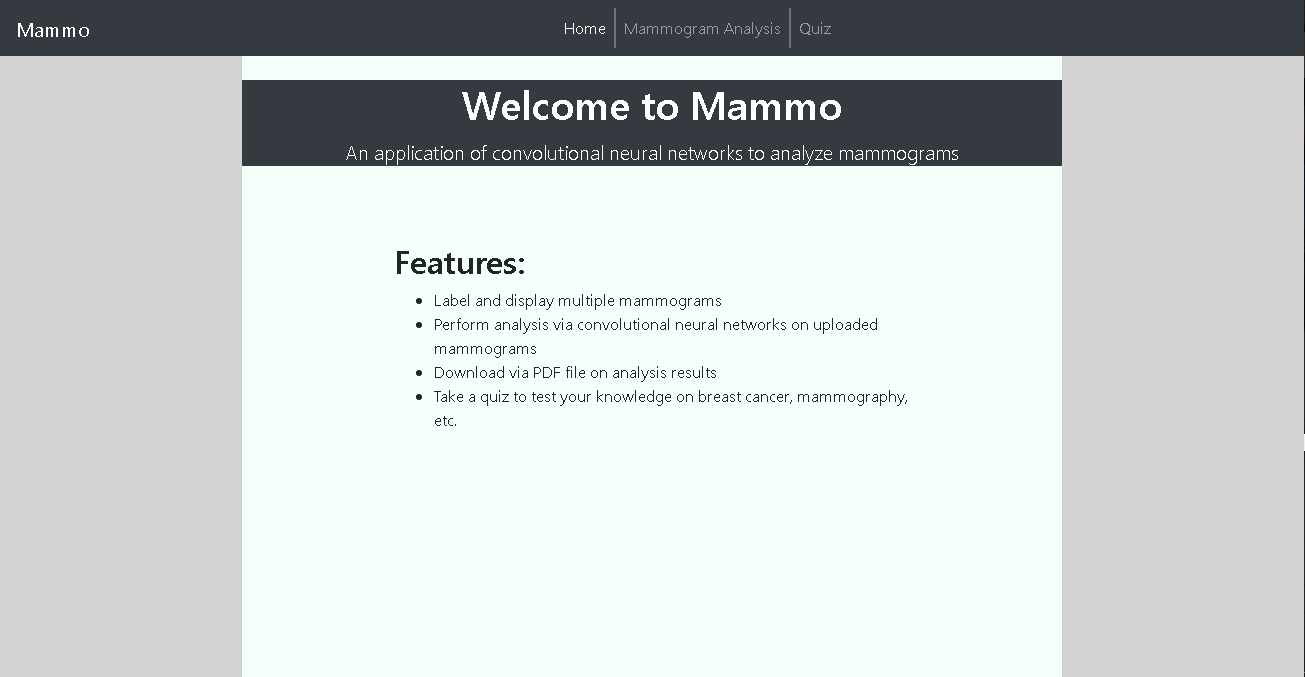
\includegraphics[scale=0.5]{images/mammoHome.png}
	\caption{Mammo home page, Mammo}
  	\label{fig:mammoHome}
\end{figure}

\subsection{Mammogram Analysis}

\subsubsection{Uploading Mammograms}
\qquad Figure \ref{fig:uploadMammograms} shows that a user has fully uploaded his chosen mammograms. A user may do this through the "Add Images" button at the top of the left sidebar or by just dragging and dropping files from his/her directory.

\begin{figure}[h]
	\centering
  	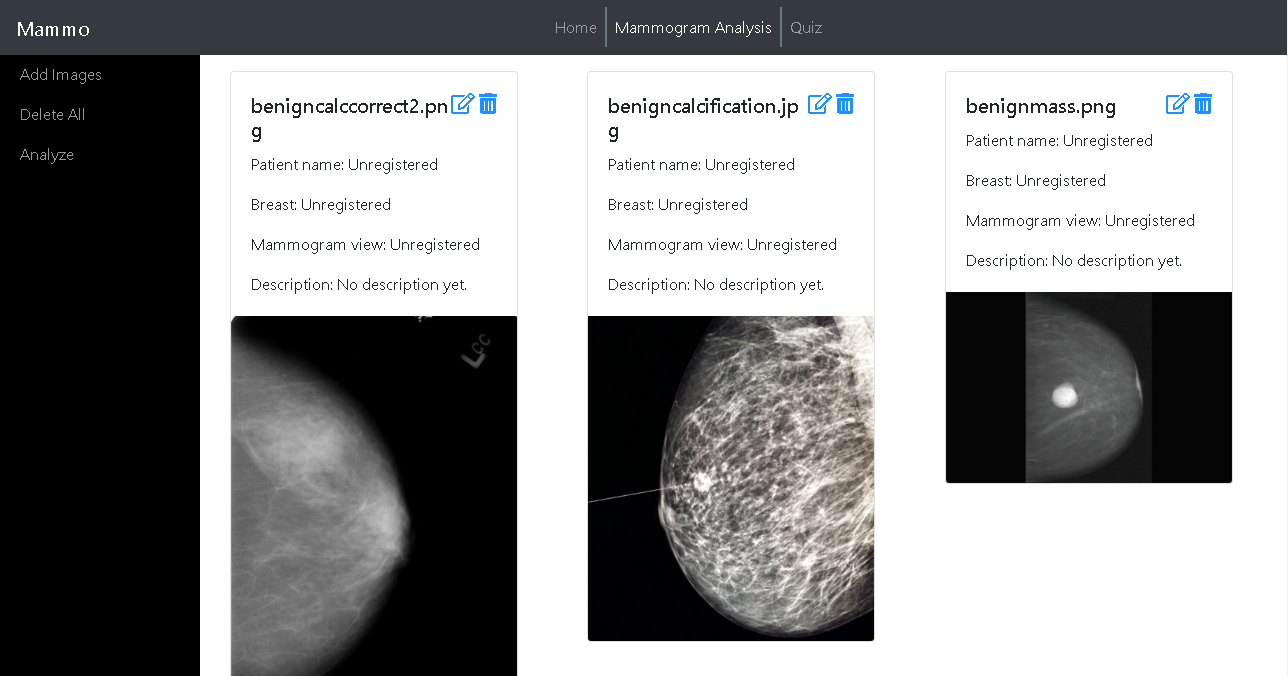
\includegraphics[scale=0.5]{images/uploadMammograms.png}
	 \caption{Three uploaded mammograms, Mammo}
  	\label{fig:uploadMammograms}
\end{figure}

\subsubsection{Editing and Deleting Mammograms}
	\qquad The mammograms are uploaded with unregistered metadata that is up for the user to edit. A user may edit the mammograms by clicking the edit icon present at the upper right of the mammogram cards, or he may simple click on the picture of the mammogram as shown figure \ref{fig:editMammograms}. Also, a user may delete the mammogram by pressing the delete icon next to the edit. Moreover, a user may delete all the mammograms uploaded by the "Delete All" button on the sidebar. Also, a user must specify the region of interest to be analyzed by the CNN module. A user may leave the metadata entries blank, but he must choose a region of interest and save it.

\begin{figure}[h]
	\centering
  	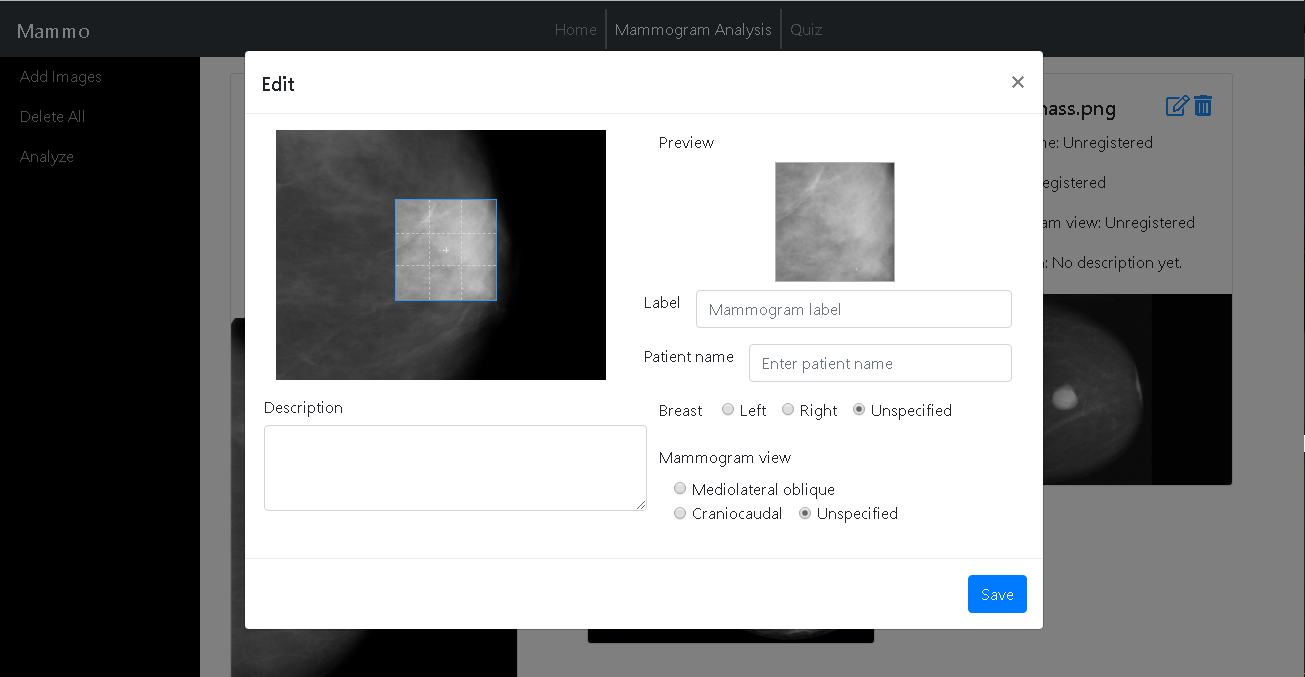
\includegraphics[scale=0.5]{images/editMammograms.png}
	 \caption{Editing metadata of the mammogram, Mammo}
  	\label{fig:editMammograms}
\end{figure}


\subsubsection{Analyzing the Mammograms}
	\qquad After the user has entered the necessary patient data, he/she may then proceed to have the mammograms analyzed by the "Analyze Mammograms" on the sidebar (see figure \ref{fig:uploadMammograms}). It may take a long time to process the mammograms. Figures \ref{fig:mammogramAnalysis1} and \ref{fig:mammogramAnalysis2} show the analysis made by the CNN module. A "Generate PDF" functionality is present for the user to save the results as PDF (see figure \ref{fig:mammogramPDF}).

\begin{figure}[h]
	\centering
  	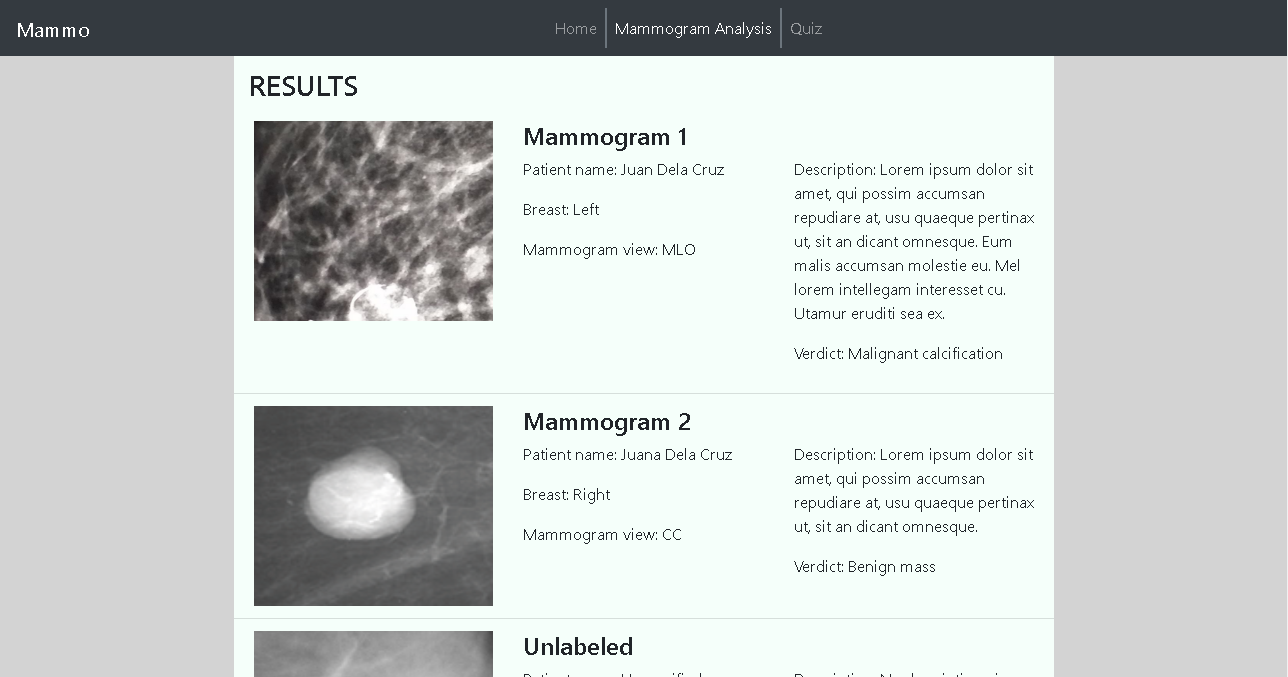
\includegraphics[scale=0.5]{images/mammoAnalysis1.png}
	 \caption{Results of the analysis made by the CNN module part 1, Mammo}
  	\label{fig:mammogramAnalysis1}
\end{figure}

\begin{figure}[h]
	\centering
  	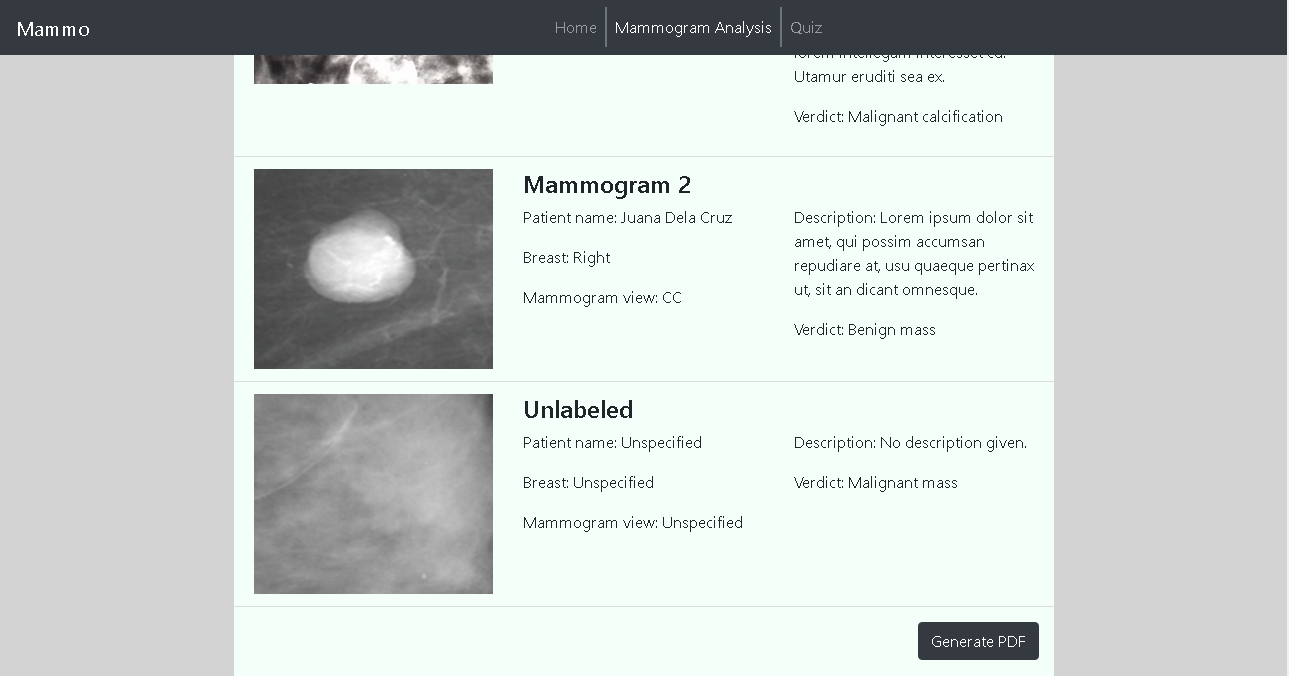
\includegraphics[scale=0.5]{images/mammoAnalysis2.png}
	 \caption{Results of the analysis made by the CNN module part 2, Mammo}
  	\label{fig:mammogramAnalysis2}
\end{figure}

\begin{figure}[h]
	\centering
  	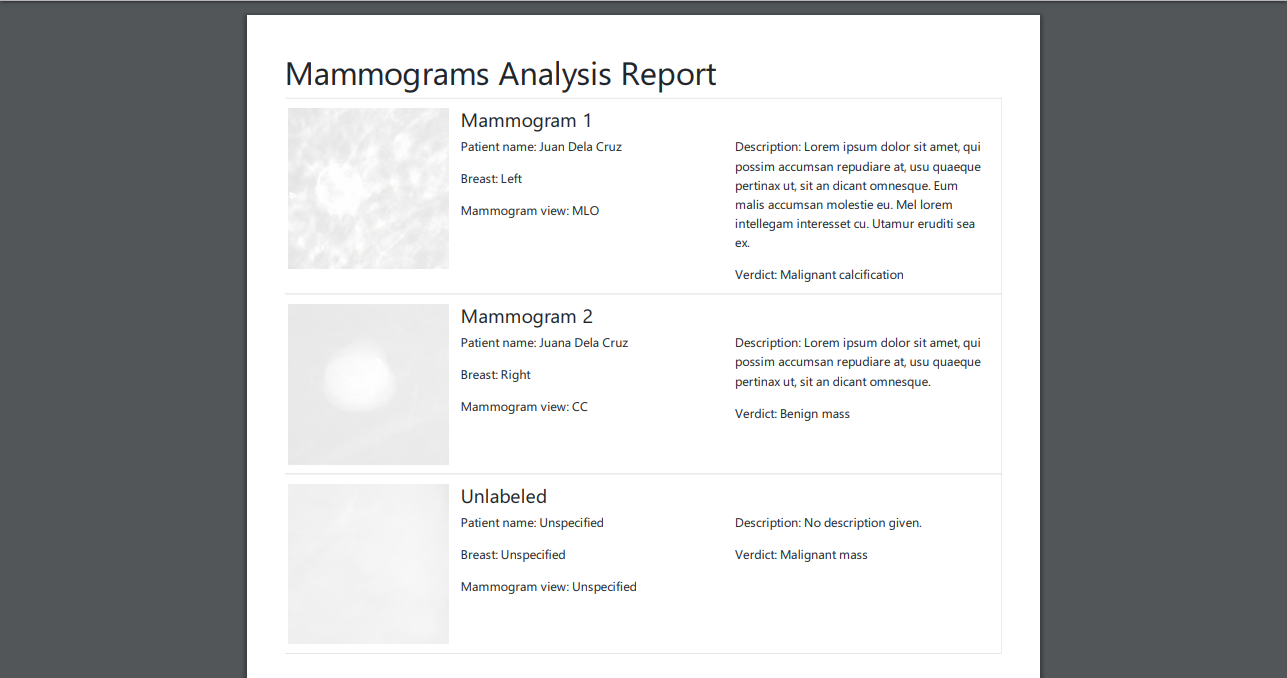
\includegraphics[scale=0.5]{images/mammogramPDF.png}
	 \caption{A generated PDF file of Mammogram Analysis Report, Mammo}
  	\label{fig:mammogramPDF}
\end{figure}

\subsection{Quiz}

\subsubsection{Taking the Quiz}
\qquad A user or a student/trainee has the option to take a randomly-generated 10-item pop quiz regarding breast cancer, mammography, treatment, etc. (see figure \ref{fig:mammogramExam}).

\begin{figure}[h]
	\centering
  	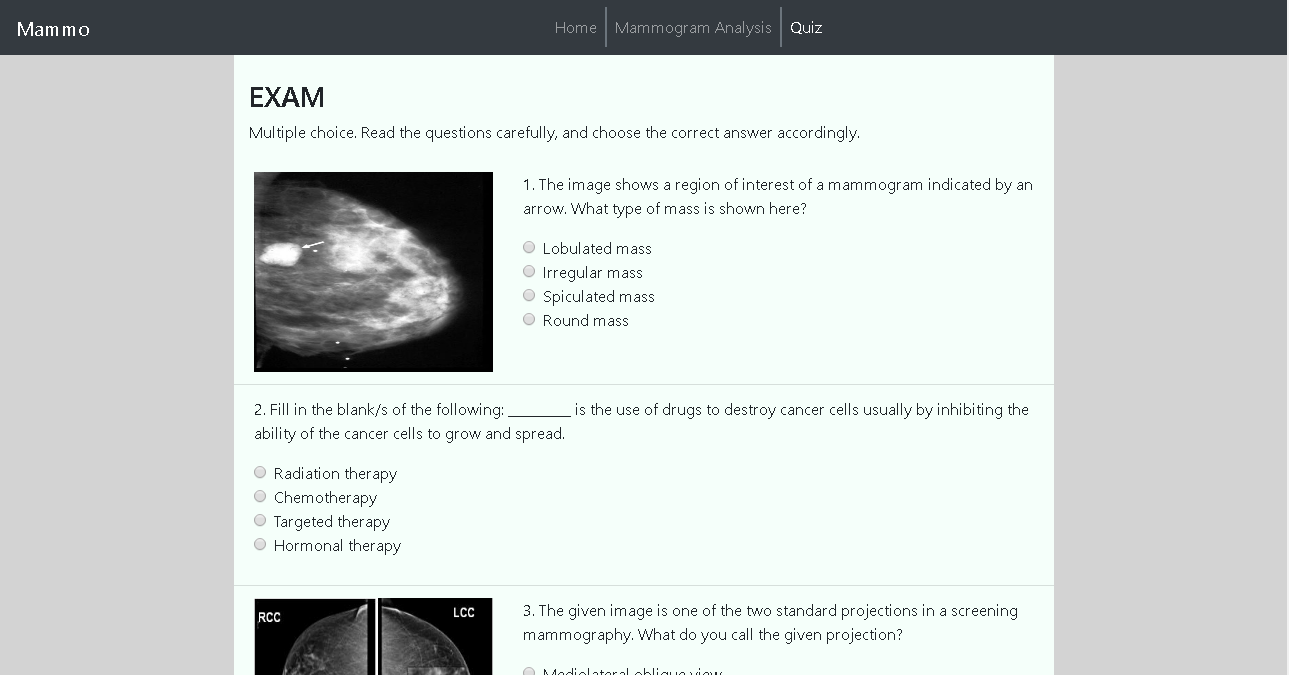
\includegraphics[scale=0.5]{images/mammogramExam.png}
	 \caption{A sample of the quiz, Mammo}
  	\label{fig:mammogramExam}
\end{figure}

\subsubsection{Quiz Results}
\qquad After the user has answered the questions and reviewed the answers, he/she may submit the quiz for evaluation by the "Submit" button seen in figure \ref{fig:submitQuiz}. The user's score and the correct answer are seen in figure \ref{fig:quizResults}.

\begin{figure}[h]
	\centering
  	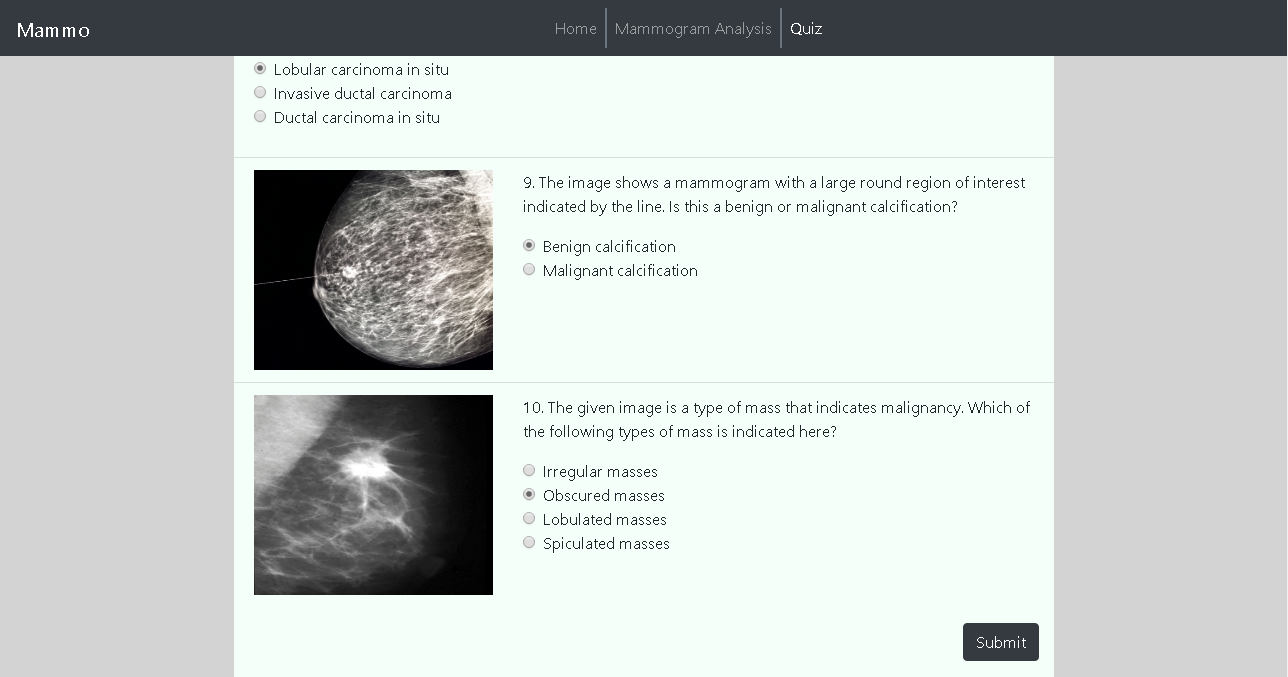
\includegraphics[scale=0.5]{images/submitQuiz.png}
	 \caption{Submit the quiz, Mammo}
  	\label{fig:submitQuiz}
\end{figure}

\begin{figure}[h]
	\centering
  	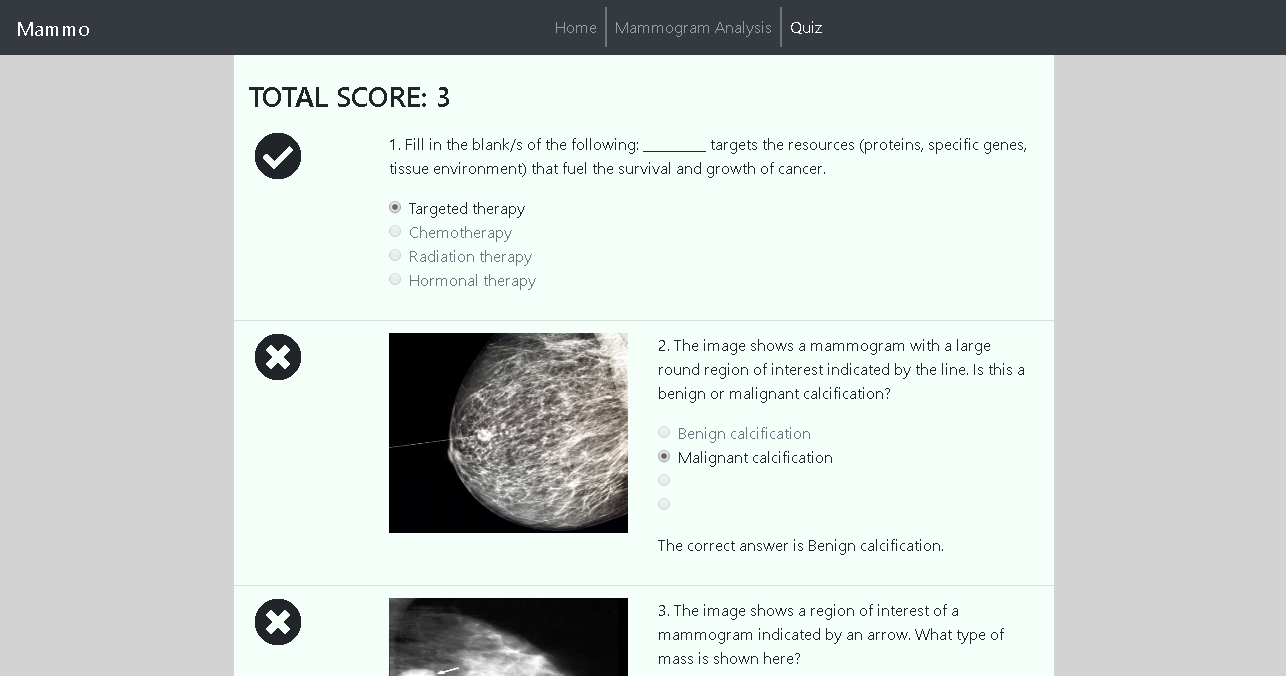
\includegraphics[scale=0.5]{images/quizResults.png}
	 \caption{Results of the quiz, Mammo}
  	\label{fig:quizResults}
\end{figure}

\clearpage
\clearpage